\documentclass{article}
\usepackage[paperwidth=210mm,paperheight=297mm, top = 30mm, bottom = 30mm]{geometry}
%\usepackage[hangul]{kotex}
\usepackage{kotex}
\usepackage[utf8]{inputenc}
\usepackage{enumitem}
\usepackage{indentfirst}
\usepackage{graphicx, subcaption, tikz}
\usepackage{amsmath, amssymb, amsthm, amsfonts, bm}

\title{2020 Spring MAS365 Numerical Analysis HW6}
\author{20160650 채지석}
\date{\today}

\setlist{  
  listparindent=\parindent,
  %parsep=0pt,
}

\newtheorem{prob}{Problem}

\newcommand{\set}[1]{\left\{ {#1} \right\}}
\newcommand{\vecx}{\boldsymbol{x}}
\newcommand{\mat}[1]{\boldsymbol{#1}}
\newcommand{\mata}{\boldsymbol{A}}
\newcommand{\matb}{\boldsymbol{B}}
\newcommand{\rr}{\mathbb{R}}
\newcommand{\nn}{\mathbb{N}}
\newcommand{\zz}{\mathbb{Z}}
\newcommand{\cc}{\mathbb{C}}
\newcommand{\qq}{\mathbb{Q}}
\newcommand{\norm}[1]{\left\lVert#1\right\rVert}
\newcommand{\card}[1]{\left\lvert#1\right\rvert}
\newcommand{\posdef}{\succ\mat{0}}
\newcommand{\psd}{\succeq\mat{0}}
\newcommand{\trace}{\text{trace}}
\newcommand{\comment}[1]{}
\newcommand{\problem}{\begin{prob}\end{prob}}
                    

\begin{document}

\section*{Computer Assignment}
The program which does the required is submitted via KLMS along with this document. For various values of \texttt{n}, the program first computes the cubic spline $S(x)$ with knots $\set{x_0, x_1, \dots, x_n}$. This is done by computing the moments using the system of linear equations learnt in class, then computing the coefficients of the cubic polynomial from the moments, ordinates, and knots. Then the program computes the error $f(x) - S(x)$ at the $41$ equidistant points. \par 
The computed cubic splines are printed out, in a matrix as the following figure. 
\begin{center}
    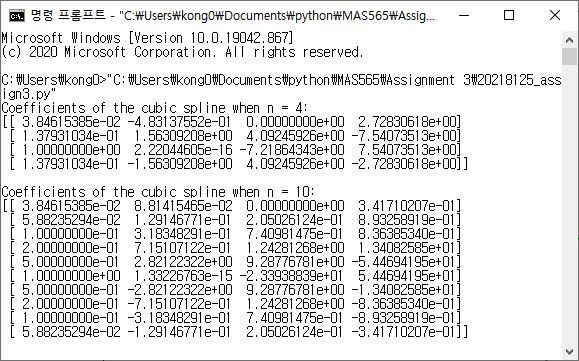
\includegraphics[width=0.8\linewidth]{console.JPG}
\end{center}\begin{center}
  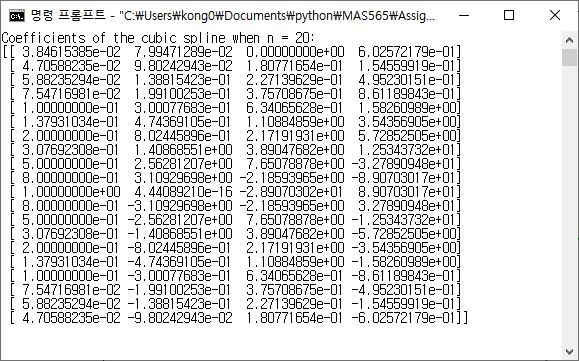
\includegraphics[width=0.8\linewidth]{console2.JPG}
\end{center}
The resulting matrix contains the list of coefficients of the cubic polynomial for each subintervals. For example, the first row of the first matrix should be interpreted as that the cubic spline when $n=4$ on $[x_0, x_1] = [-1.0, -0.5]$ coincides with the cubic polynomial
\[
0.03846 -0.4831 x + 0 x^2 + 2.728x^3.
\] We have computed natural splines, so the coefficient of the quadratic term for the leftmost subinterval is always $0$, as the results show. \par  
The errors $f(x) - S(x)$ at $41$ equidistant points are plotted, as the following figure, so that we can visualize and easily see how good the cubic splines are for various values of $n$. 
\begin{center}
    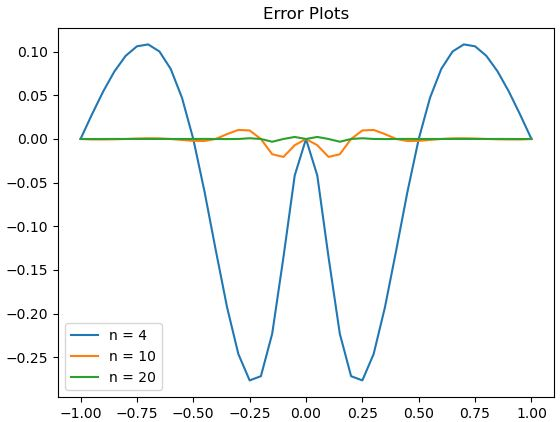
\includegraphics[width=0.85\linewidth]{3313.JPG}
\end{center} \par 
The figure indicates that the interpolation accuracy increases with the number of knots.

\end{document}